\chapter{Object Versioning} \label{chapter:APPROACH}

This chapter introduces our approach to recovering development states of object-oriented programming systems that consists of objects.
Our approach is based on alternative, version-aware references that manage versions of objects transparently.
As a concrete solution for the Lively Kernel, we present a design based on using proxies for implementing the version-aware references.


\section{Version-aware References} \label{sec:APPROACH:1}

The development state in a programming system such as the Lively Kernel consists of the state of objects.
In different versions of the system, the available objects have different states. 

\begin{figure}[h]
    \centering
    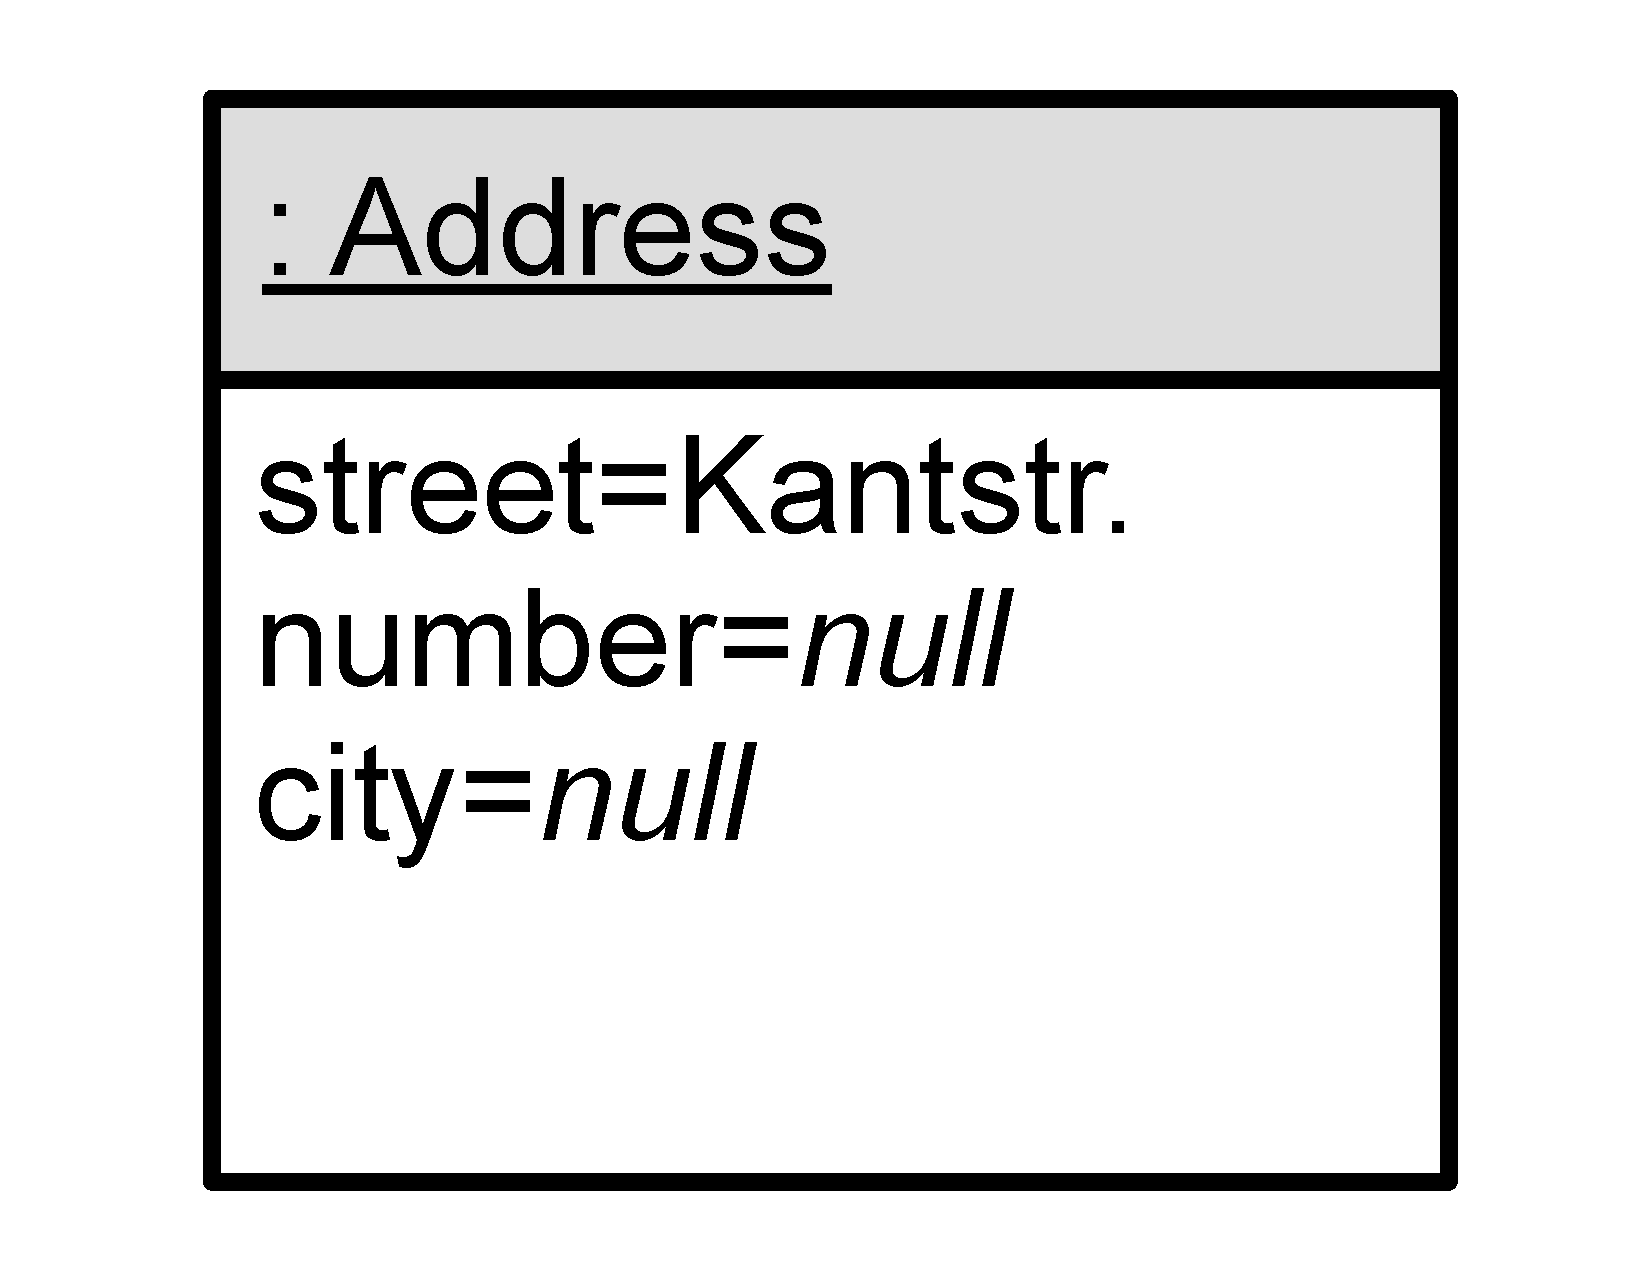
\includegraphics[width=0.3\textwidth]{figures/4_approach/1_singleObject.pdf}
    \caption{An \emph{address} object with three properties.}
    \label{fig:SingleObject}
\end{figure}

For example, an object could represent an address.
The state of such an \emph{address} object could be as shown in Figure~\ref{fig:SingleObject}.
If the object now gets values for its \lstinline{city} and \lstinline{number} fields, the object's state would be changed.
As the address object's state is part of the development state, changing the address object also changes the development state.
If we call our first development state version \emph{v1} and the one after making changes to the object version \emph{v2}, the state of the address object is different for the two versions of the system, as shown in Figure~\ref{fig:ObjectChanged}.

\begin{figure}[h]
    \centering
    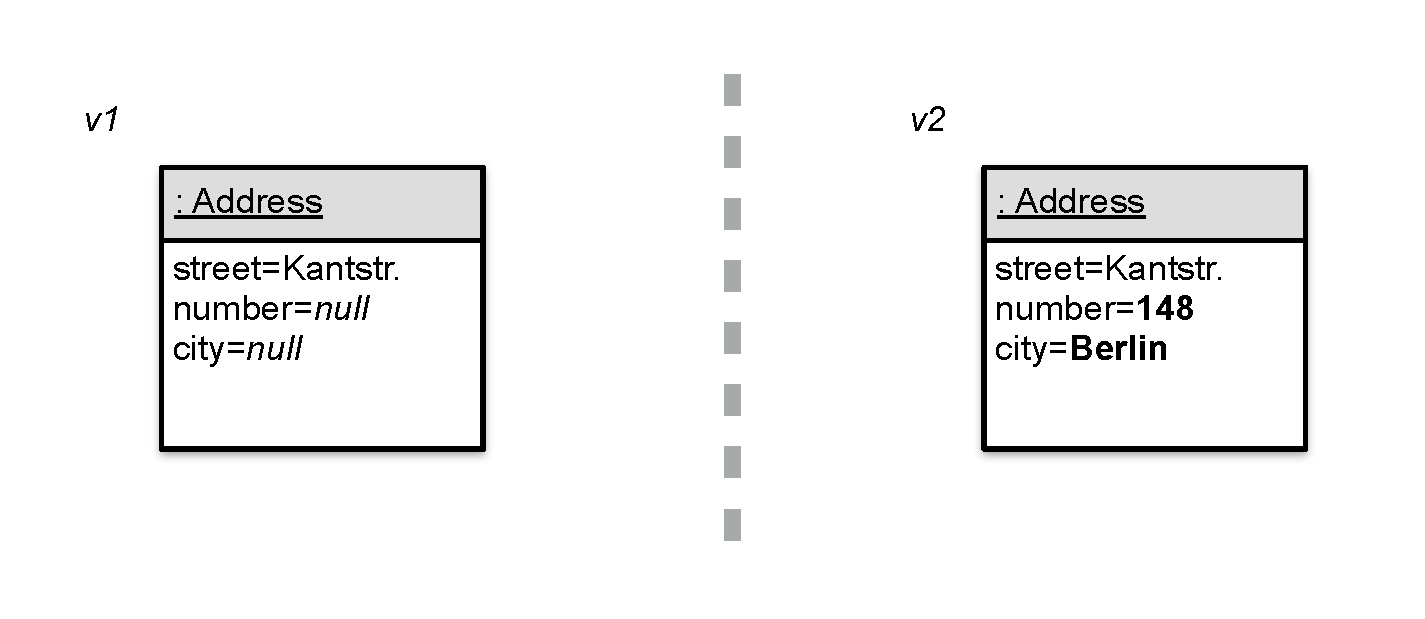
\includegraphics[width=0.7\textwidth]{figures/4_approach/2_objectChange.pdf}
    \caption{Two versions of the same \emph{address} object in two versions of the system.}
    \label{fig:ObjectChanged}
\end{figure}

To preserve the previous development state when making changes, the system needs to preserve the previous states of its objects.
For this reason, with object versioning, versions of objects are preserved, while changes are made to new versions of the objects.
A version of an object is, in the simplest case, a full copy of an object---also an object.
That is, when the address object is changed in version \emph{v2} of the system, the system does not change the orginal address object but a copy of it.
Subsequentely, there are now two address objects in version \emph{v2}, as shown in Figure~\ref{fig:VersionPreserved}.
One of these object versions holds the original state, while the other holds the state that the object has in version \emph{v2} of the system.

\begin{figure}[h]
    \centering
    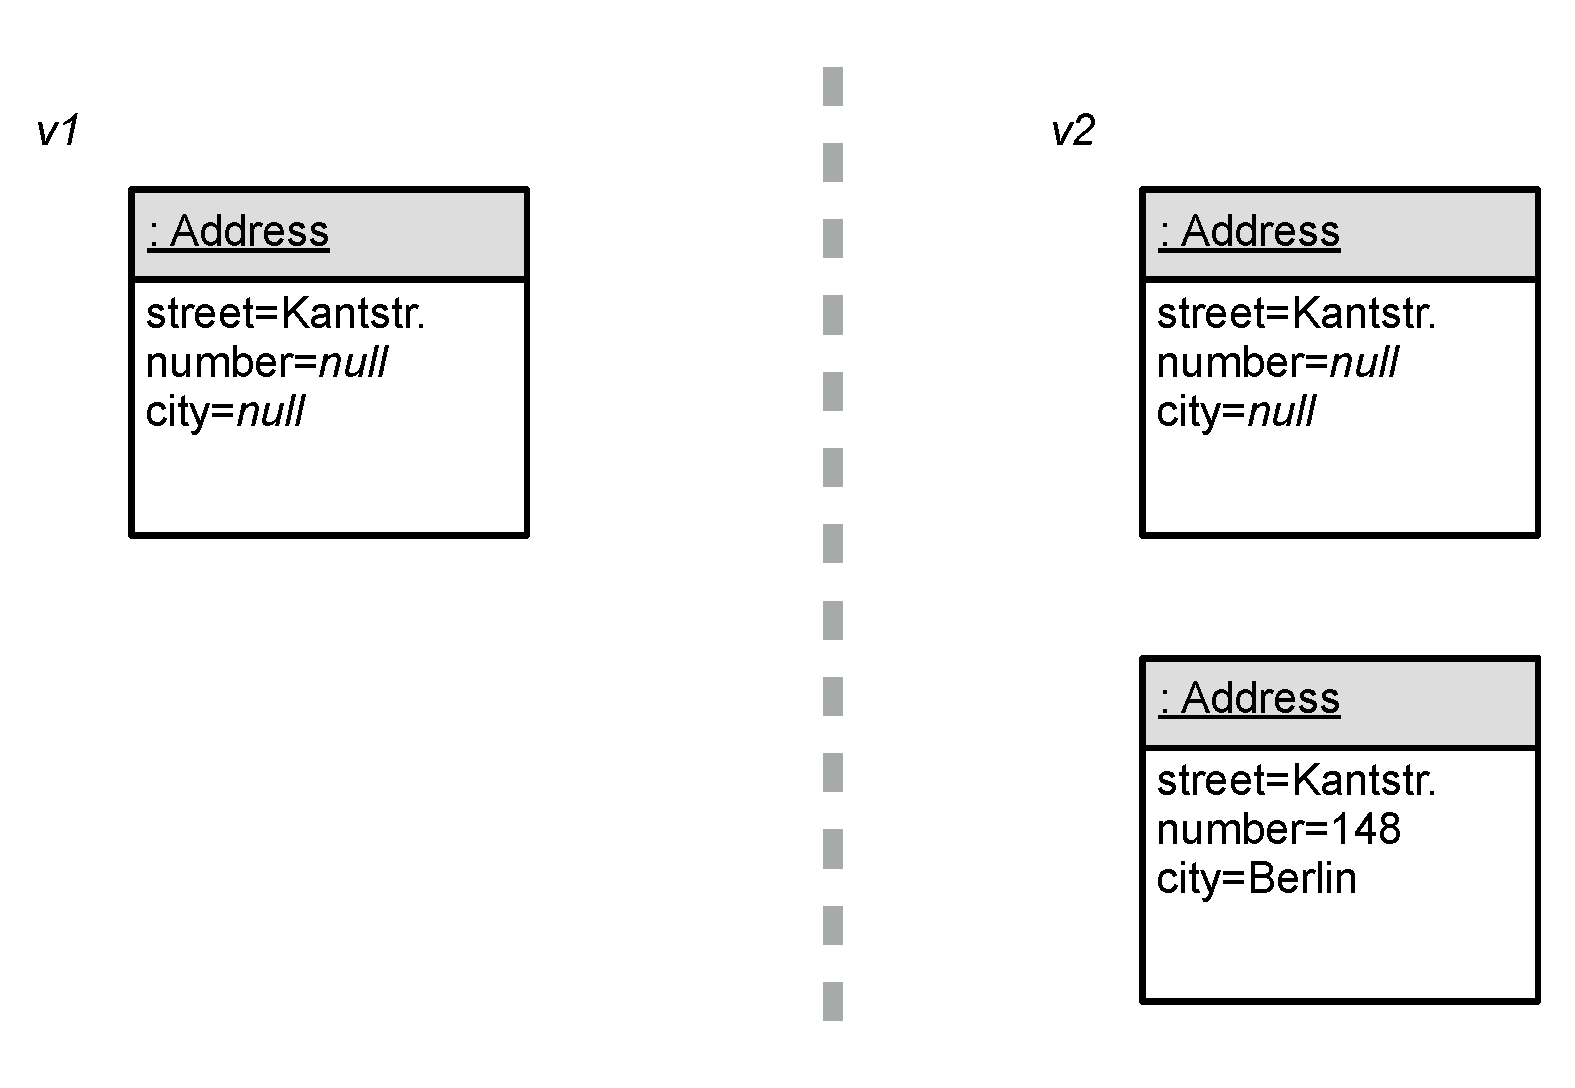
\includegraphics[width=0.7\textwidth]{figures/4_approach/3_previousVersionPreserved.pdf}
    \caption{Preserving the previous version of the \emph{address} object.}
    \label{fig:VersionPreserved}
\end{figure}

For the single address object, there are now two versions of the object.
These versions hold no knowledge to which version of the system they belong.
They also store no indication that one of them is a copy of the other one.
At the same time references to objects are not changed when simply copying an object.
For example, there could have been a person object with an \lstinline{address} property referring to the address object.
This reference will still be referring to the original address object, even in version \emph{v2} of the system, as shown in Figure~\ref{fig:ReferenceFixedToPreviousVersion}.

\begin{figure}[h]
    \centering
    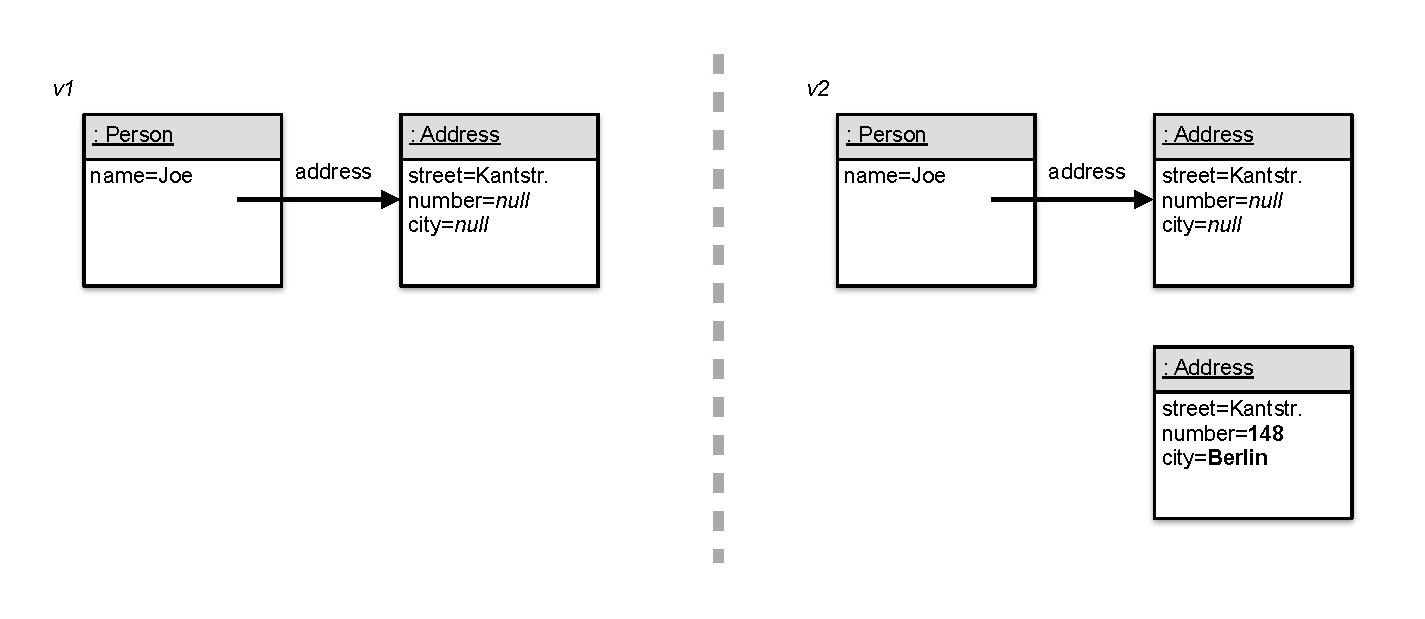
\includegraphics[width=\textwidth]{figures/4_approach/4_referenceToPreviousVersion.pdf}
    \caption{A reference refers to the previous version of the \emph{address} object.}
    \label{fig:ReferenceFixedToPreviousVersion}
\end{figure}

That is, even after adding values to the fields of the address object, the following statement would still return true when \lstinline{aPerson} is the person object:

\iffalse
\begin{verbatim}\fi
\begin{code}[lst:example]{}{float}
aPerson.address.city === null
\end{code}
\iffalse
\end{verbatim}\fi

For this, our approach to object versioning uses \emph{version-aware references}.
Version-aware references know the available versions for an object and always resolve to one of those.
Moreover, version-aware references know which version of an object belongs to which version of the runtime.
Using context information the version-aware references resolve to the correct version dynamically.
That is, none of the versions is hard-wired to be the active version.

Otherwise, the version-aware references behave like ordinary references.
They can be assigned to variables, object fields, and also get passed around.

When the \lstinline{person} object now holds a version-aware reference as its \lstinline{address} property, it can resolve the reference to the current version.
That is, the version-aware reference knows both versions of the address object and would resolve to the second version in version \emph{v2} of the system, as depicted in Figure~\ref{fig:VersionAwareReferenceFollowingVersion2}.

\begin{figure}[h]
    \centering
    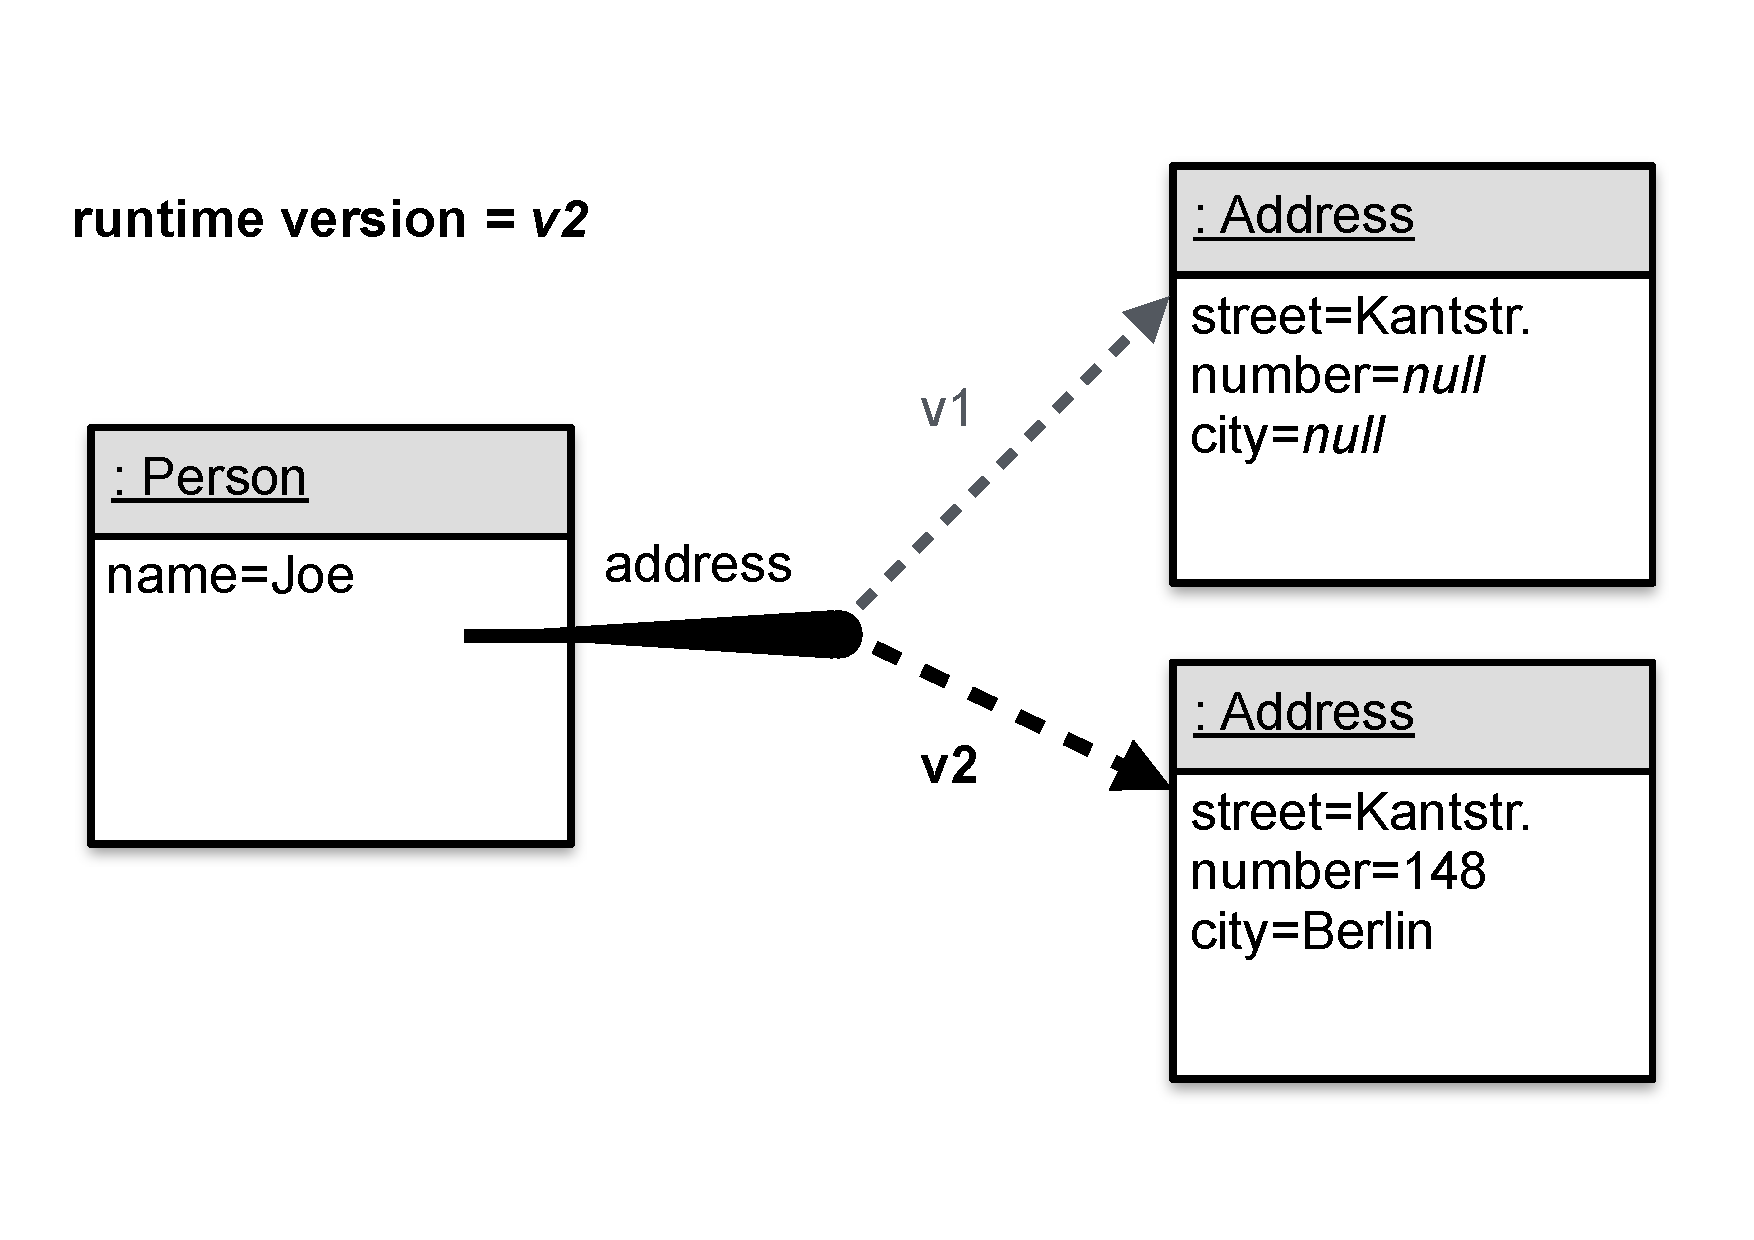
\includegraphics[width=0.5\textwidth]{figures/4_approach/5_versionAwareReferenceFollowingVersion2.pdf}
    \caption{A version-aware reference relates the \emph{person} object to both versions of the \emph{address} object.}
    \label{fig:VersionAwareReferenceFollowingVersion2}
\end{figure}

In the same way, multiple version-aware references can be resolved together as a path through a graph of versions.
The version-aware references all choose versions of objects that belong to the same state and that form the object graph of a particular runtime state.

Figure~\ref{fig:ObjectGraphWithWithReferencesResolvedAlongVersion2} shows an object graph that incorporates the previous example.
The previously presented \lstinline{person} object is here the \lstinline{CEO} property of a \lstinline{company} object.
While the example currently indicates that version \emph{v2} is active, it also shows a version \emph{v1} and a version \emph{v2}.
In version \emph{v1}, the company's CEO has incomplete address information.
In version \emph{v3}, the company has a new CEO.

\begin{figure}[h]
    \centering
    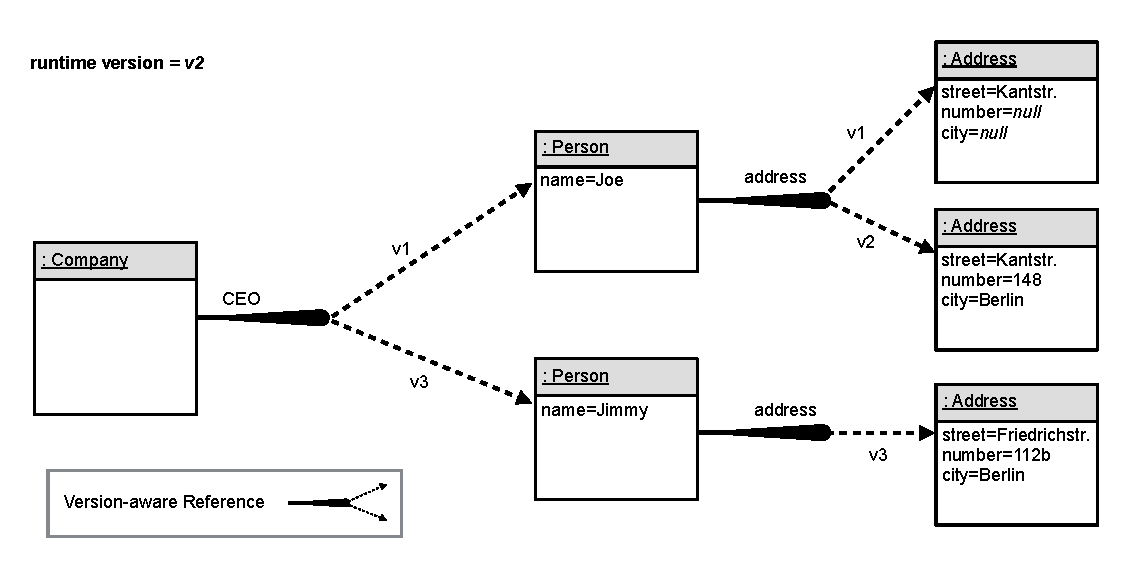
\includegraphics[width=\textwidth]{figures/4_approach/6_objectGraphWithVersonAwareReferences.pdf}
    \caption{Three versions of a \emph{company} object, in which objects are connected through version-aware references.}
    \label{fig:ObjectGraphWithWithReferencesResolvedAlongVersion2}
\end{figure}

Given \lstinline{aCompany} refers to the company object, the following statement would refer to three different values depending on the current version of the system:

\iffalse
\begin{verbatim}\fi
\begin{code}[lst:example]{}{float}
aCompany.CEO.address.number
\end{code}
\iffalse
\end{verbatim}\fi

Evaluating the statement in version \emph{v1} would return the value \lstinline{null}, in version \emph{v2} the value \lstinline{148}, and in version \emph{v3} the value \lstinline{112b}.
That is, to change the version of the system only the version identifier---the context information used by version-aware references to decide to which version they should resolve---needs to be changed.
To undo the changes to the address object and re-establish the previous development state, the version identifier would just need to be set to \emph{v1} again.

This example also shows that the version identifiers can be related: the information that version \emph{v1} is the predecessor of version \emph{v2} can be used to resolve to the \emph{v1}-version of an object when no \emph{v2}-version is available.
This allows to only create new versions of objects when necessary.

The version identifier needs to be accessible to version-aware references.
It could be available globally, to have a single active version of the runtime, but could also be scoped more locally such as thread-local or in the dynamic scope of a code block.
It should, however, not be changed while object relations in an object graph are transitively resolved.
That is, the version-aware references involved in evaluating the previously presented example statement should be resolved together for one version identifier.

To be able to actualy re-establish development states with our approach now, two requirements need to be fullfilled:
First, all mutable objects of the programming runtime need to be accessed via version-aware references.
Second, the version of the runtime that should be re-established need to have been preserved.
That is, the versions of objects reflecting the specific development state need to be available for the references.

With our approach, specific versions can be preserved.
That is, not every state is recoverable, but specific states need to be preserved.
Programmers could preserve versions explicitly or the programming system could do this implicitly.
When the programming system automatically preserves versions, each programmer actions could implicitly create a new version of the system.
This way, programmers can undo and redo the changes associated with specific and rememberable actions.
Further, programmers could always undo actions, regardless of whether they preserved a version in anticipation of recovery needs or not.



% TODO: add a summary of the benefits of the version-aware references..
% 
% % DESIGN IMPLICATIONS / RATIONALE

% % design for fine-grained histories (many small versions): costs spread / constant execution overhead (time): (dynamic references) instead of re-wiring hard references, copy-on-write instead of copying all objects for a version
% % ++ copy-on-write is also an optimization of memory requirements: incremental versioning on the granularity of objects
% % ++ objects are kept as readily usable objects in memory (instead of storing versions on disk)
% 
% 
% Version-aware references allow to change versions without stopping the system.
% First, the version-aware references resolve dynamically to particular versions based on context information.
% Only this context information has to be changed to have all references resolve to another version, without updating any of the version-aware references.
% Second, preserving a new version of the runtime also happens incrementally.
% Instead of saving versions of all objects that make up the runtime, when the development state is to be preserved, new versions of objects can be created only when objects subsequentely change.
% Before such writes the previous object states continue to reflect the current state and can, thus, be read for following versions until written.
% This way, as \emph{objects} are copied on writes, versioning happens automatically on the granularity of objects.
% For the same reason, resulting histories can also be fine-grained as for each version only changed objects need to be copied.
% 
% 
% % Further, creating many versions is not expected to interrupt the programmers workflow as the execution costs of preserving a version is spread: Instead of copying all objects the moment a version should be preserved, objects are only copied when and in the moment they are subsequentely changed.
% % In general, the approach aims to distribute the cost for object versioning: besides incrementally saving a version, switching the active version is also not interruptive as the version-aware references resolve to versions dynamically and all versions reside as objects in application memory.
% 







\section{Using Proxies for Version-aware References} \label{sec:APPROACH:2}








% 1. HOW-PROXIES

For a concrete solution for the Lively Kernel, we use proxies for version-aware references.
Instead of actually using \emph{alternative references}, proxies are referred to by \emph{ordinary references} and delegate to versions. 
That is, the proxies stand-in for multiple versions, intercept all access, and forward to the correct version.

Proxies allow a language-level solution for alternative references.
First, even though an implementation at the level of the virtual machine would probably have performance advantages, using proxies for a first implementation is considerably less effort.
Second, there are many different JavaScript engines and many different versions of those in use today.
Using proxies an implementation can work in many engines without adapting each one.

Figure~\ref{fig:ProxyBasedVersionAwareReference} exemplifies how a proxy implements a version-aware reference between a \lstinline{person} object and the two versions of its \lstinline{address} property.
The \lstinline{person} holds an ordinary reference in its \lstinline{address} slot, which, however, refers to a proxy.
The proxy in turn knows which versions are available for the \lstinline{address} object.

\begin{figure}[h]
    \centering
    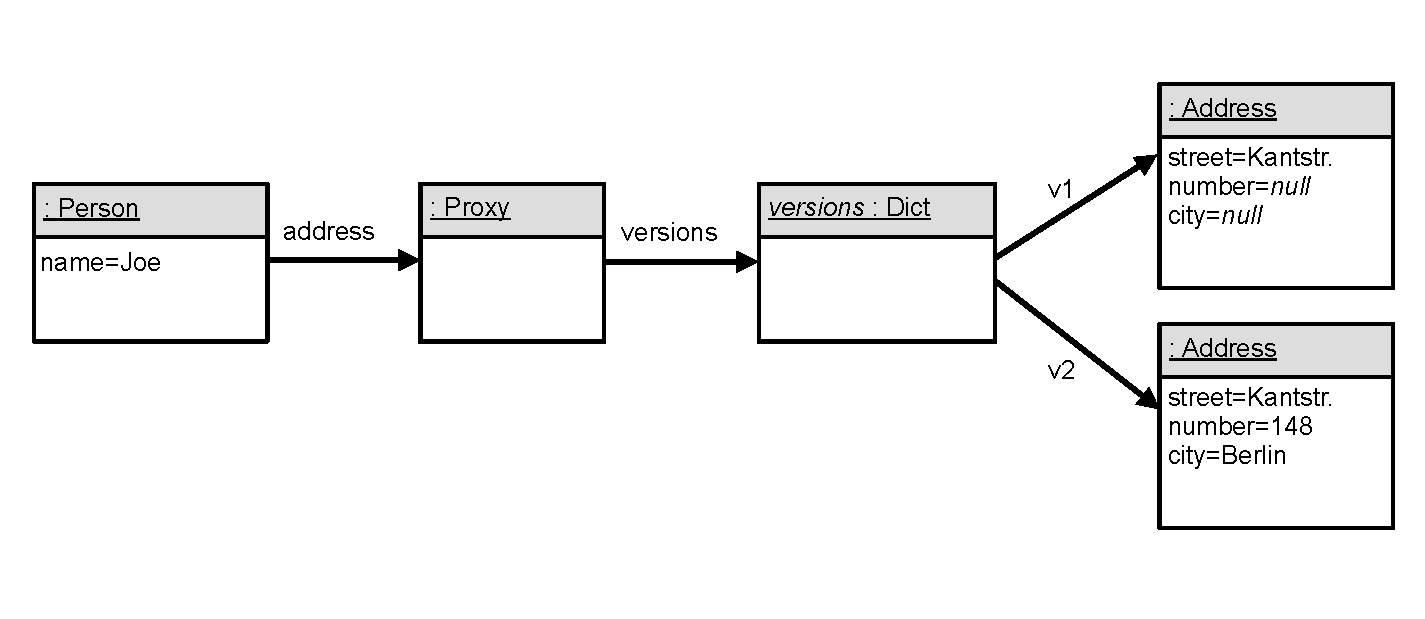
\includegraphics[width=\textwidth]{figures/4_approach/7_proxyBasedVersionAwareReference.pdf}
    \caption{Using a proxy as version-aware reference between the \emph{person} object and its versions of the \emph{address} object.}
    \label{fig:ProxyBasedVersionAwareReference}
\end{figure}

When the \lstinline{address} property of the \lstinline{person} object is used, the proxy needs to forward the access transparently to the correct version.
Even if the \lstinline{address} property is a proxy, reading, for example, the proxy's \lstinline{city} property needs to return the string \lstinline{'Berlin'} in version \emph{v2} of the system as indicated by Figure~\ref{fig:ProxyBasedVersionAwareReference}.
That is, evaluating the following statement needs to return true in version \emph{v2}, given \lstinline{aPerson} refers to the \lstinline{person} object:

\iffalse
\begin{verbatim}\fi
\begin{code}[lst:example]{}{float}
aPerson.address.city === 'Berlin'
\end{code}
\iffalse
\end{verbatim}\fi

Note that the statement does not include any code that is aware of versions.
In particular, it does not read a specific version from the table of available versions.
Instead, the proxies need to forward the property read to a specific version transparently.

For this, the proxies need to fulfill these three responsibilities to implement version-aware references:
\begin{enumerate}
    \item They need to know which versions are available for a particular object.
    \item They need to choose one particular version among all available dynamically using context information.
    \item They need to delegate object access transparently to a chosen version.
\end{enumerate}

The proxies required for an implementation of this design are proxies that can intercept all kinds of access and response arbitrarily.
Such proxies, also referred to as \emph{virtual objects}~\cite{VanCutsem2010PDP}, do not stand-in for a specific object, but are able to forward access to any object.

Further, besides having proxies that can intercept and forward access and fullfill the stated responsibilities, the proxies also need to be used consistently.
Ordinary references that usually refer directly to an object now need to refer to the proxy that stands-in for the versions of the object instead.

To use proxies consistently for all mutable objects, proxies are created and returned for new objects right when objects are created.
All expressions that create new objects return proxies for those objects instead.
For this, we transform the code before execution and wrap object literals as well as constructor functions into proxies.
Additionally, we also have proxies always return proxies for return values.
Then, when proxied constructors are used, the proxies return proxies for the new objects.

The reference to the actual object---or, more precisely, the initial version of an object---is only available to the proxy, while the reference to the proxy gets passed around instead of it.
For this reason, all references that would usually point to the same object now point to the same proxy, so that proxies also provide object identity.
Checks that would usually compare an object with other objects now compare a proxy with other proxies.



% TODO: how are versions preserved: global versions + copy-on-write

% versions are created.. by programmers or the system..


% global version information: linear: versions with predecessors and successors, maybe with a figure..

% % + FIGURE of the versions, haha!!

% These information are used to decide to which particular versions of objects proxies are to delegate at any moment.
% Given which version of the runtime is currently active, the proxies can choose the corresponding version of the object.
% 
% 
% This way, the proxies transitively all delegate to objects that make up the state of the entire runtime as it was at a particular moment---when the version of the runtime was last active.
% To preserve a development state, the version of the runtime just has to be changed.
% 
% 
% 
% The version of the runtime can be global in JavaScript as JavaScript engines use only a single thread and cooperative scheduling.
% There is, therefore, no way to change which version of each object should be used while a path through an object graph is already partly resolved.






% TODO: summary


% When all objects are referred to through the proxies now, 

% by references that dynamically and transparently choose one particular version of the objects as they were at a particular moment.
% When these references are then used for all mutable objects of a runtime, the entire runtime state can be preserved and re-established.













% Vorsicht.. TEXT LEICHEN.. !!!!





% Proxies allow a language-level implementation of alternative references in JavaScript:
% Without requiring adaptions to the virtual execution engines, proxies can be inserted to stand-in for objects---so references that usually point directly to objects point to proxies instead---and these proxies can provide versioning information and behavior.
% These proxies are, thus, an alternative to using ordinary references to directly refer to objects.
% That is, some objects can, potentially, still be referred to directly, while objects that should be versioned should be accessed only though proxies.
% In our solution for the Lively Kernel, nearly all objects are only accessed through proxies, except for some particular \emph{root objects} that are not required to be versioned but potentially do refer to other objects via version-aware references.

% rationale for using proxies:
% (as opposed to providing alternative references on virtual machine-level: language-level solution as there are many different engines used for executing JavaScript (which would all require implementations of version-aware references to have the Lively Kernel with recovery support for all users. also implementation in JavaScript is easier (especially for a first prototype) and does not have to go through any formal review or standardization process, which language features added to JS engines usually do))









% Proxies hold multiple versions of an object.
% They can transparently delegate access to one particular among many versions.
% They are also referred to consistently instead of the object.
% This allows to have and use particular versions of particular objects.
% However, to enable programmers to undo and redo arbitrary changes to the entire development state, our solution needs to preserve and choose versions of all objects in a coordinated way and be able to establish particular versions of the entire runtime instead of just of single objects.
% Our solution to this is declaring versions of the runtime and, then, annotating versions of objects with the version of the runtime they are part of.





% When these proxy-based version-aware references can know the versions of an object and are used consistently to access mutable objects, the proxies only need to know which versions to choose at a given moment and when to copy current versions to preserve particular runtime states.
% For this, the runtime is enhanced with a global version identifier representing the current version, which the proxies use to annotate newly proxied objects or new versions of objects with and also to choose the correspondingly annotated versions when accessing proxies.
% This then is enough to provide a simple undo/redo for the Lively Kernel.





% TRANSPARENCY of version-awareness

% transparency requirements: transparent for programmers: programmers should not have to adapt their programs, programmers should not have to distinguish between version-aware and ordinary references

% Version-aware references behave transparently, just like a usual reference to the current version of the object would.
% They are assigned to variables and get passed around, and, under usual circumstances, programmers do not have to be aware of them.
% Firstly, programmers should not be required to adapt their programs to use version-aware references.
% Instead version-aware references should be provided consistently by the programming system.
% Secondly, there should be no direct references to particular versions of objects.
% Programmers should not have to distinguish between version-aware references and direct references, while having both direct references to one particular version and a version-aware reference that always refers to current version could also introduce inconsistencies.






% 
% Versions of objects are also just JavaScript objects and, thus, also in memory.
% The proxies, in this solution, also contain the versions of the object they stand-in for.
% This way, when a proxy, which stands in for all versions of conceptually one object, is no longer referred to from anywhere, all versions of an objects are reclaimed by the ordinary JavaScript gargage collector.